\setlength{\baselineskip}{0.5cm}
\chapter{Berichte}

Sie k�nnen sich in diesem Abschnitt verschiedene Statistiken generieren lassen,
um sich einen �berblick �ber die angefallenen Kosten und Ausgaben zu verschaffen.

\section{Kostenstelle}
\label{bericht_kostenstelle}

\begin{figure}
	\centering
	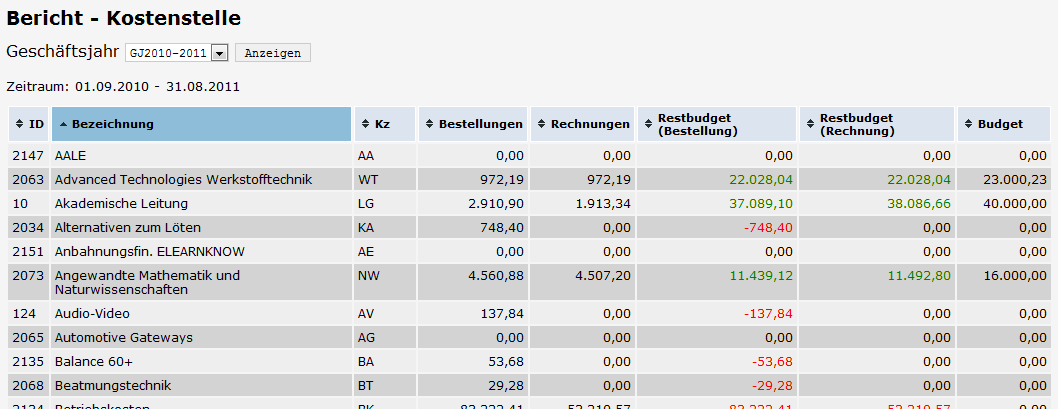
\includegraphics[width=1\textwidth]{bericht_kostenstelle.png}
	\caption{�bersicht �ber die Kostenstellen}
	\label{bericht_kostenstelle_screenshot}
\end{figure}

Nach der Auswahl des gew�nschten Gesch�ftsjahres aus dem Drop-Down Men�, wird Ihnen eine Auswertung �ber alle vorhandenen Kostenstellen erstellt.
Den verschiedenen Spalten (welche Sie durch einen Klick auf die �berschrift auch sortieren k�nnen) k�nnen Sie zB. die Bestellsumme oder das Restbudget entnehmen.

\section{Tags}
\label{bericht_tags}

Mithilfe der Checkboxen k�nnen Sie die gew�nschten Kostenstellen markieren, welche bei der Statistik ber�cksichtigt werden sollen.
W�hlen Sie anschlie�end das gew�nschte Gesch�ftsjahr aus dem Drop-Down Men� und klicken Sie auf \textit{Anzeigen}.

\begin{figure}
	\centering
	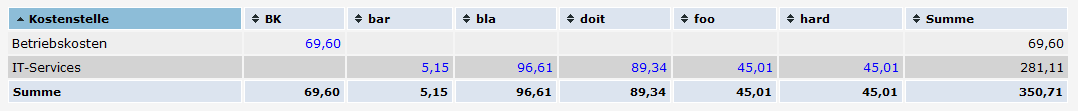
\includegraphics[width=1\textwidth]{bericht_tags.png}
	\caption{Auswertung der verwendeten Tags}
	\label{bericht_tags_screenshot}
\end{figure}

Abbildung \ref{bericht_tags_screenshot} zeigt ein Beispiel einer solchen Auswertung.
In den einzelnen Spalten sehen Sie alle, in der jeweiligen Kostenstelle verwendeten, Tags.
Der Summenzeile k�nnen Sie dann mit einem Blick entnehmen, wieviele Ausgaben in Bestellungen mit dem entsprechenden Tag get�tigt worden sind.

\info{Wenn Sie bei einer Bestellung oder Bestellposition mehrere Tags definiert haben, werden diese auch bei der Auswertung entsprechend mehrmals ber�cksichtigt und zur Gesamtsumme addiert. Zus�tzliche Tags verf�lschen also die Gesamtsumme.}

\section{Aufteilung}
\label{bericht_aufteilung}

Hier k�nnen Sie, einstellbar f�r das gew�nschte Gesch�ftsjahr, die Bruttokosten, aufgeteilt auf die einzelnen Organisationseinheiten, einsehen.
W�hlen Sie aus dem Drop-Down das gew�nschte Studiensemester und klicken Sie auf \textit{Anzeigen}, um das jeweilige Gesch�ftsjahr einsehen zu k�nnen.



